\documentclass[conference]{IEEEtran}
\IEEEoverridecommandlockouts
\usepackage{cite}
\usepackage{amsmath,amssymb}
\usepackage{graphicx}
\usepackage{booktabs}
\usepackage{textcomp}
\usepackage{url}
% keep command names and the ISA name from breaking across lines
\newcommand{\cmd}[1]{\mbox{\texttt{#1}}}
\hyphenation{RISC-V}
\renewcommand{\topfraction}{0.92}
\renewcommand{\bottomfraction}{0.85}
\renewcommand{\textfraction}{0.06}
\renewcommand{\floatpagefraction}{0.75}

\begin{document}

\title{Verifying the RISC-V IOMMU: An Open Environment\\and What Fault Injection Says About It}
\author{\IEEEauthorblockN{Maulik Timbadiya}
\IEEEauthorblockA{\textit{Independent Researcher}}}
\maketitle

\begin{abstract}
The RISC-V IOMMU specification reached version 1.0 and open RTL implementations
have followed, but the leading one ships with no testbench and there is no
published verification methodology for this class of device. We report an open,
licence-free verification environment for it: 1{,}144 lines of SystemVerilog
that drive all four AXI interfaces, serve the device's implicit page-table,
command and fault-queue accesses from a memory model, and check every
translation against an independent software walker. It builds in 2.4~s and runs
56 checks in 5~ms under Verilator. We evaluate the environment by injecting
eleven semantically meaningful IOMMU defects into the RTL. An early suite
detected four of nine; the survivors named concrete blind spots---page-table
permission bits, reserved-bit encodings, second-stage translation---and tests
written to close them raised detection to eleven of eleven. We report two
findings about the IP, including that with the fault queue disabled a faulting
device leaves the IOMMU unresponsive, and one about methodology: a
protocol-violating bus driver in our own testbench manufactured three plausible
and entirely false IP defects.
\end{abstract}

\begin{IEEEkeywords}
IOMMU, RISC-V, functional verification, fault injection, address translation.
\end{IEEEkeywords}

\section{Introduction}
An IOMMU confines a DMA-capable device: it translates the addresses the device
emits and enforces the permissions of the domain that owns it. A defect in it is
a containment failure. The RISC-V IOMMU specification is now at version~1.0 and
open implementations exist, the most complete being the IP published by Zero-Day
Labs~\cite{rviommu}, whose own documentation states it ``is not formally
verified'' and is ``very likely to have bugs.'' It ships no testbench; its
makefile runs Verilator in \texttt{--lint-only} mode.

Verification of RISC-V \emph{cores} is well served~\cite{riscvdv,corevverif},
and address-translation \emph{ordering} has been studied for CPU
MMUs~\cite{coatcheck,transform,rtlcheck}, but we are not aware of published work
on verifying a RISC-V IOMMU. This paper reports what building such an
environment takes, and measures how much of the device it exercises by injecting
defects rather than by counting coverage.

\section{Background}
A device issues a transaction carrying a device identifier. The IOMMU walks a
device-directory table in memory to obtain a device context, which names the
translation structures for that device: a first-stage table (Sv39), a
second-stage table (Sv39x4), or neither, in which case the transaction passes
through untranslated. The result is cached in an IOTLB and the context in a
directory cache. Because those caches are filled from memory the host also
writes, software invalidates them through a command queue using
\cmd{IOTINVAL.VMA}, and learns when invalidation has taken effect using
\cmd{IOFENCE.C}. Faults append a record to a fault queue and abort the
transaction.

Three properties make this awkward to drive. The stimulus is bus transactions on
one port while the quantity under test---the translated address---appears on a
\emph{different} port that the testbench must implement as a slave. Most
behaviour depends on data structures in memory, so no stimulus is meaningful
until valid directory and page-table images exist. And the caches make behaviour
history-dependent: the same transaction is correct or incorrect depending on
what was invalidated before it.

\section{Related Work}
Verification of RISC-V cores is well served. \texttt{riscv-dv}~\cite{riscvdv}
generates constrained-random instruction streams, and
\texttt{core-v-verif}~\cite{corevverif} provides UVM environments with
reference-model co-simulation. Both target cores, both rely on a commercial
simulator for their UVM components, and neither addresses an IOMMU.

Address translation has been approached from the ordering side. COATCheck models
memory ordering at the hardware--OS interface including translation
events~\cite{coatcheck}; TransForm synthesises litmus tests for such
``transistency'' models~\cite{transform}; RTLCheck verifies that RTL satisfies
the microarchitectural axioms a consistency proof assumes~\cite{rtlcheck}. All
concern a CPU's MMU and the software that maintains it. None targets a
device-side IOMMU, and none builds a functional verification environment for
one---which is the gap this paper addresses, and a narrower slice of which---the
ordering obligation an IOMMU owes to an unmap path---we treat
separately~\cite{companionB}.

Fault injection as a measure of suite adequacy is long established in software
as mutation testing and has been applied to hardware description languages to
assess verification quality. We use it not as a novel technique but because it
answers the question that matters for a new environment: not how many lines were
executed, but which defects would survive.

\section{Device Under Test}
We target the Zero-Day Labs IP at commit \texttt{18ad30a}: 75 SystemVerilog
files, 25{,}778 lines. It implements device-directory walks, Sv39 first-stage
and Sv39x4 second-stage translation, an IOTLB and directory caches, a command
queue and a fault queue; it does not implement ATS. It exposes four AXI4
interfaces: a device-request slave, a completion master on which translated
transactions leave, a master for implicit accesses, and a programming slave.

One observation is immediate: the IP cannot be linted as published. Its register
map includes \texttt{common\_cells/assertions.svh}, which the repository does not
vendor, and supplying the upstream lowRISC header fails because that header
defines \texttt{ASSERT\_RPT} with two arguments where the IP's RTL uses one. We
forward the path to the IP's own bundled header, after which it lints clean.

\section{Environment}

\begin{figure*}[!t]
\centering
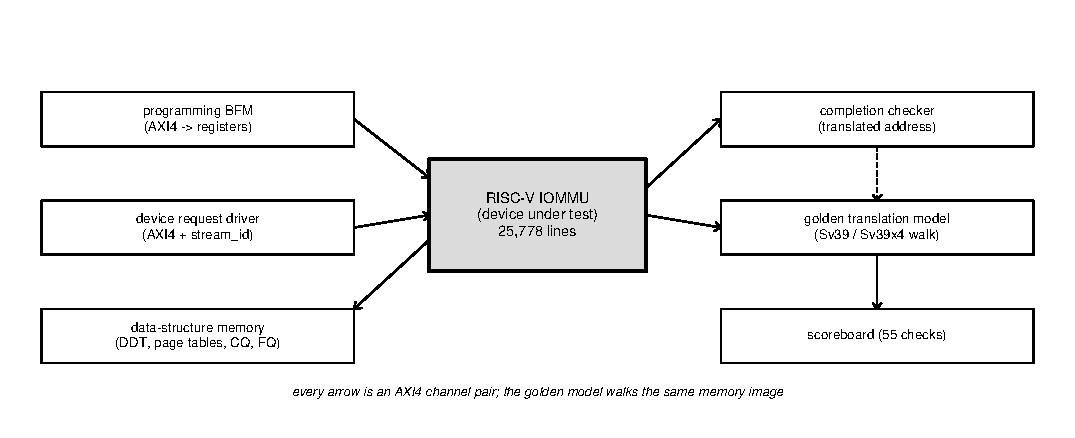
\includegraphics[width=\textwidth]{figures/figA1_env.pdf}
\caption{Environment structure. The translated address is observed on the
completion port, which the testbench implements as a slave, and compared against
an independent walk of the same memory image.}
\label{fig:env}
\end{figure*}

Fig.~\ref{fig:env} shows the structure: a programming driver, a data-structure
memory model serving every implicit access from a 512~KiB image, a device
request driver carrying a device identifier, a completion checker implementing
the master port as a slave, and an independent Sv39 walker that reads the same
memory image and predicts the address each transaction should produce.

Three details proved necessary. Register accesses must support both widths: the
\texttt{ddtp} register commits only when both of its 32-bit halves have been
written, and sub-word accesses must carry their true byte address or they write
the neighbouring register. The command queue is a ring whose tail index must
wrap; omitting the wrap left the device with an out-of-range tail and silently
disabled invalidation while every earlier test still passed. And both drivers
determine completion by counting channel handshakes, not by sampling a
\texttt{valid} level, because after a faulting transaction a level-sampling
driver mistakes a stale response for its own.

\section{Test Suite}
The suite is 56 checks: register access; \texttt{ddtp} programming and
\texttt{Bare}/one-level directory modes; first-stage translation including 32
random mappings checked against the walker and an IOTLB hit that performs no
walk; second-stage Sv39x4 translation; caching and invalidation, including
address-scoped invalidation, invalidate-all, \cmd{IOFENCE.C} completion and a
concurrent-traffic case with 24 accesses in flight; and faults, covering invalid
contexts, unmapped addresses, \texttt{ddtp}$=$\texttt{Off}, fault-queue records,
and page-table entries with the accessed, dirty, user or valid bit clear or a
reserved bit set. \begin{table}[!t]
\caption{Test areas}
\label{tab:areas}
\centering\footnotesize
\begin{tabular}{lrl}
\toprule
Area & \# & Representative check \\
\midrule
Register interface    & 4  & 4-byte write takes effect \\
Directory, modes      & 8  & context read from right address \\
First-stage Sv39      & 7  & 32 random maps match walker \\
Second stage Sv39x4   & 4  & GPA maps to expected SPA \\
Caching, invalidation & 13 & no stale entry after fence \\
Faults, permissions   & 19 & dirty bit clear faults a write \\
\midrule
Total                 & 55 & (plus 1 precondition check) \\
\bottomrule
\end{tabular}
\end{table}

\begin{figure}[!t]
\centering
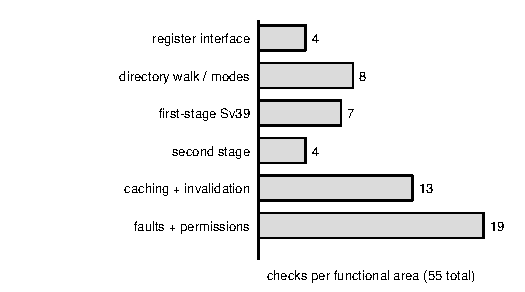
\includegraphics[width=\columnwidth]{figures/figA3_checks.pdf}
\caption{Distribution of the functional checks.}
\label{fig:checks}
\end{figure}

Table~\ref{tab:areas} and Fig.~\ref{fig:checks} summarise the areas. The suite builds in 2.4~s and runs
in 5~ms, which is what makes the fault-injection campaign cheap enough to repeat
after every change.

\section{Fault-Injection Evaluation}

\begin{table}[!t]
\caption{Injected defects and detection}
\label{tab:mutants}
\centering\footnotesize
\begin{tabular}{llc}
\toprule
 & Injected defect & Detected \\
\midrule
M1  & first-stage PTE valid bit ignored          & yes \\
M2  & PTE accessed bit ignored                   & yes \\
M3  & PTE dirty bit ignored on stores            & yes \\
M4  & PTE user bit ignored (second stage)        & yes \\
M5  & PTE reserved-bit check removed             & yes \\
M6  & \texttt{ddtp}$=$\texttt{Off} no longer blocks traffic & yes \\
M7  & \texttt{Bare} decoded as a normal mode     & yes$^{\dag}$ \\
M8  & first-stage enable inverted                & yes \\
M9  & IOTLB invalidation does not clear entries  & yes \\
M10 & command-queue head never advances          & yes \\
M11 & invalidate-all clears only the first entry & yes \\
\bottomrule
\end{tabular}
\\[2pt]
\footnotesize $^{\dag}$detected as a hang: the suite fails to complete.
\end{table}

\begin{figure}[!t]
\centering
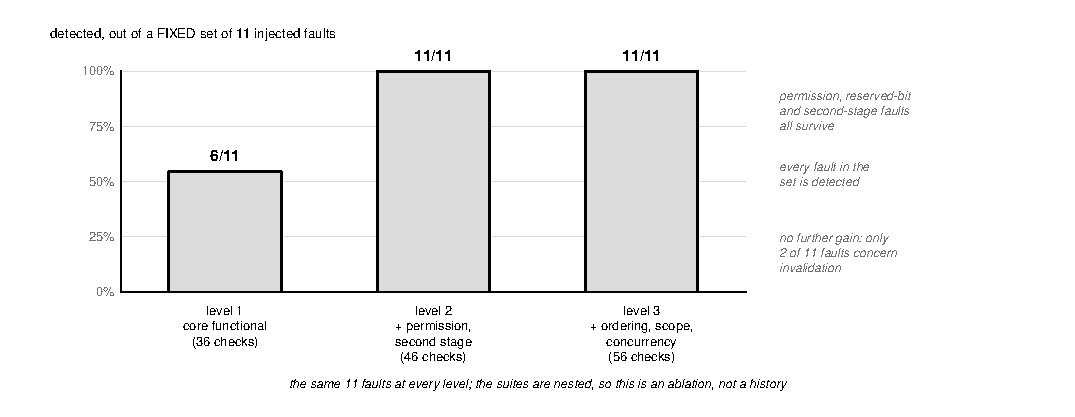
\includegraphics[width=\columnwidth]{figures/figA2_mutation.pdf}
\caption{Detection as the suite grew. The surviving defects named the blind
spots; the tests written to close them raised detection.}
\label{fig:mut}
\end{figure}

Each defect is one scripted edit to a private copy of the RTL; the suite is
rebuilt and rerun, and a defect counts as detected if any check fails.
Table~\ref{tab:mutants} gives the final result. The trajectory in
Fig.~\ref{fig:mut} is the useful part: the first suite of 34 checks detected
four of nine usable defects, and the survivors were systematic rather than
random---every page-table permission defect survived because our entries always
set the accessed, dirty and user bits; the reserved-bit defect survived because
we never set reserved bits; the second-stage defect survived because every test
left the second stage in \texttt{Bare} mode. Tests for those behaviours raised
detection to eleven of eleven. All 34 original checks passed on the unmodified
RTL and would have passed on an RTL missing every page-table permission check.

\section{Findings}

\subsection{A faulting device can render the IOMMU unresponsive}
With the fault queue disabled we first confirm a valid translation works, then
issue eight faulting transactions, then repeat the valid one. Four of the eight
receive a response and four receive none; the subsequent valid transaction then
fails. We report this as observed rather than as a specification violation,
since the specification's requirements for faults with a disabled queue are
weaker than for the enabled case and we did not isolate the internal cause. The
practical exposure stands regardless: software that has not yet enabled the
fault queue leaves a path by which a misbehaving device can stop the IOMMU
servicing transactions.

\subsection{A protocol-violating testbench manufactures defects}
\label{sec:false}
We recorded three reproducible defects in the IP during development: 4-byte
register writes silently dropped, \texttt{ddtp} not reprogrammable after device
traffic, and a sub-word access corrupting the next write. All three were false,
caused by two faults in our own driver. It deasserted \texttt{w\_valid} a cycle
late and so transferred two write-data beats for a single-beat burst, leaving a
spare beat queued in the device's bus bridge so every later write used the
previous transaction's data; and it masked sub-word addresses to the 8-byte
boundary, so a 4-byte write at offset \texttt{0x24} was issued at \texttt{0x20}.
We found them only by monitoring both sides of the device's internal bridge and
observing correct data entering and stale data leaving.

The stimulus side of a testbench is unverified code driving a protocol. When it
violates that protocol the device behaves strangely in ways easily attributed to
the device. Protocol checkers are routinely bound to the device under test; this
argues for binding them to the drivers too.

\section{Limitations}
The score measures detection of defects we chose and is not a general adequacy
claim. The environment exercises one directory mode, 4~KiB pages and a 64-bit
bus; superpages, three-level directories, process contexts, MSI translation and
the debug interface are untested, and the IP implements no ATS. All results come
from one simulator. The fault-queue finding is reported as observed behaviour.

\section{Reproducibility}
The environment, the fault-injection harness and the raw results are released
under a permissive licence. One command builds the environment and runs the
suite; a second reproduces the injection table. The only dependencies are
Verilator and Python, so the whole evaluation runs on a laptop in under a
minute, including all eleven rebuilds.

\section{Conclusion}
A 25{,}778-line open IOMMU shipped without a testbench and without a file needed
to lint it. An environment of 1{,}144 lines drives it end to end with free
tools, and fault injection---not coverage---revealed that a suite passing every
check would have missed every page-table permission defect. The same discipline
applied to our own drivers would have saved more time still.

\begin{thebibliography}{9}
\bibitem{rviommu} Zero-Day Labs, ``RISC-V IOMMU IP,'' commit \texttt{18ad30a}.
[Online]. Available: \url{https://github.com/zero-day-labs/riscv-iommu}
\bibitem{riscvdv} CHIPS Alliance, ``riscv-dv.'' [Online]. Available:
\url{https://github.com/chipsalliance/riscv-dv}
\bibitem{corevverif} OpenHW Group, ``core-v-verif.'' [Online]. Available:
\url{https://github.com/openhwgroup/core-v-verif}
\bibitem{coatcheck} D.~Lustig \emph{et al.}, ``COATCheck: Verifying memory
ordering at the hardware--OS interface,'' in \emph{ASPLOS}, 2016.
\bibitem{transform} N.~Manerkar \emph{et al.}, ``TransForm: Formally specifying
transistency models and synthesizing enhanced litmus tests,'' in \emph{ISCA},
2018.
\bibitem{companionB} M.~Timbadiya, ``Testing device-side invalidation ordering
in an IOMMU at RTL,'' companion paper.
\bibitem{rtlcheck} Y.~A.~Manerkar \emph{et al.}, ``RTLCheck: Verifying the
memory consistency of RTL designs,'' in \emph{MICRO}, 2017.
\end{thebibliography}

\end{document}
